\section{Schedule and risks}

\subsection{Schedule}

According to the estimated work an delivery dates, the full tracking plane will be ready for installation at July 2015. The overview of the schedule is the following:

\begin{figure}[h!]
  \centering
  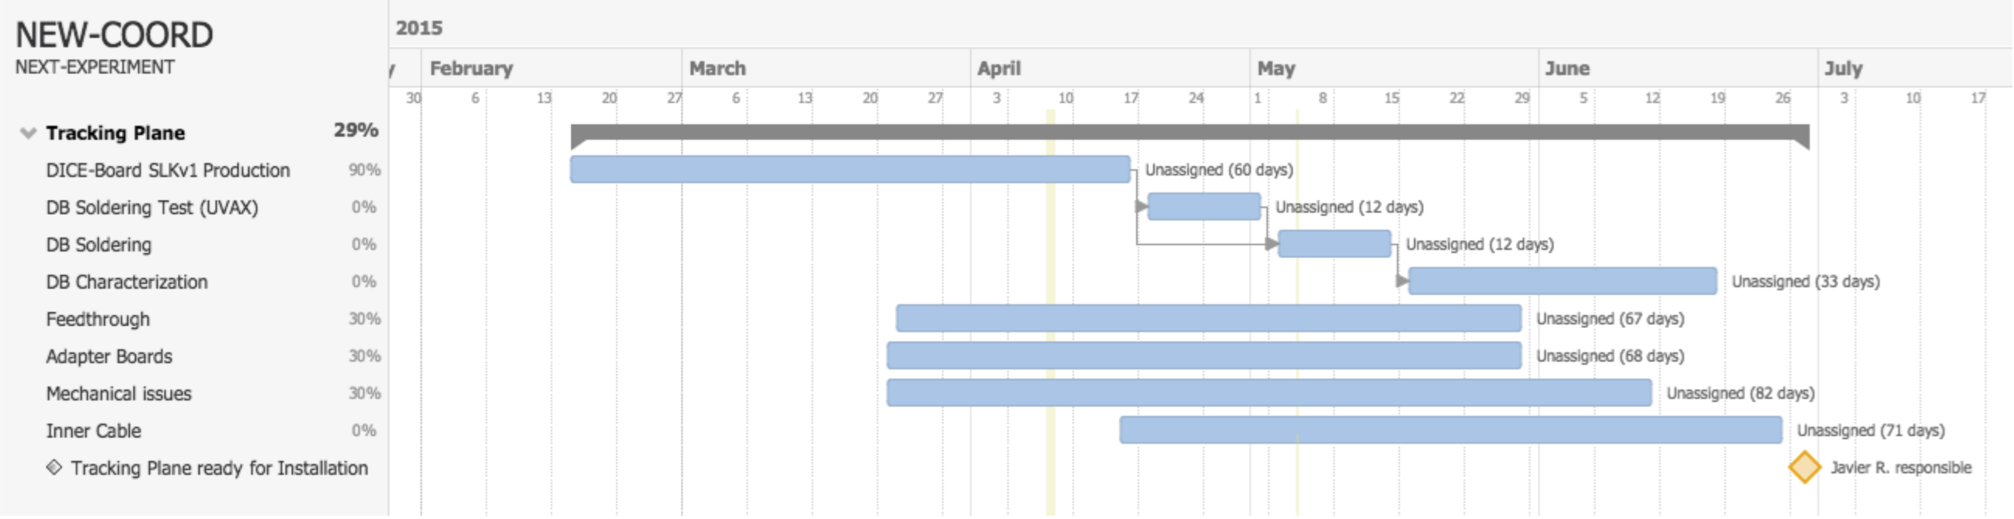
\includegraphics[width=\textwidth]{Schedule.png} 
  \caption{\textit{Estimated Tracking Plane Schedule}}
  \label{fig:schedule}
\end{figure}

As the tracking plane depends also on the field cage for working, the installation could be delayed until the field cage is done.

\subsection{Risks}

There are a lot of elements that need to be under control for the NEW tracking plane assembly, and some of them imply potential risks that can delay the installation according to schedule.

\textbf{High risks:}
\begin{itemize}
\item Inner Cables: The manufacturing of these cables has a delivery time about 2-2.5 months, and they have not been ordered yet. If they are ordered without major problems inside the term foreseen, they will arrive on time.

\item SiPM soldering: This is a difficult job, because the assembly company has to handle a large number of very small optical devices (SiPMs), and solder them to a thin flexible kapton board (DICE-Boards). There are no companies with experience, so some soldering tests must be done to be sure they can solder the whole tracking plane SiPMs.
\end{itemize}

\textbf{Low risks:}
\begin{itemize}
\item Cabling/noise: The full cabling chain from the front-ends to the SiPMs is very long and complex, and need to be tested at LSC to know the real performance. This depends also on the inner cables, that has not been produced yet and need also to be tested.
\end{itemize}

%%%%%%%%%%%%%%